\minitoc

\section{Pemrograman aplikasi GUI}

Tulisan ini ingin memamparkan bagaimana membuat sebuah aplikasi GUI sederhana dengan mudah
menggunakan Qt Creator . Aplikasi sederhana dengan fungsi  dasar tombol dan label (untuk gambar).
Jika tombol pertama di klik, maka gamabr A muncul. Jika tombol kedua di klik, maka gambar 
B muncul. Dengan contoh dasar tersebut di harapakan mamou memahamai dasar-dasar dari sebuah 
pemrograman GUI di Qt Creator yakni signal dan slot.

\subsection{Menyiapkan Proyek}

\begin{enumerate}
	\item Buka Qt Creator dan buat proyek baru. Pilih Application \textgreater{} Qt Widget Application\footnote{gunakan pilihan ini untuk membuat applikasi GUI untuk proyek masa mendatang}.
	
		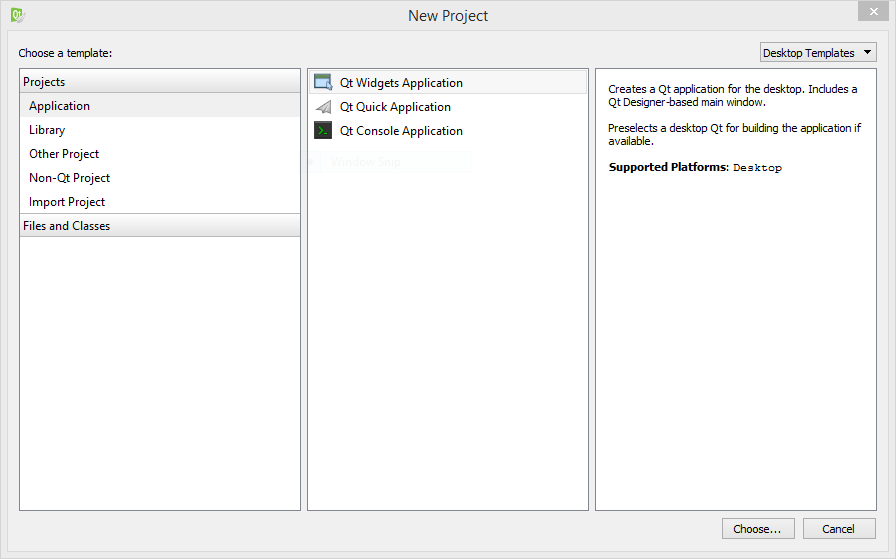
\includegraphics[width=0.8\textwidth]{../manuscript/images/Capture14-1.PNG}
		
		\item Beri nama Aplikasi yang akan di buat
		
		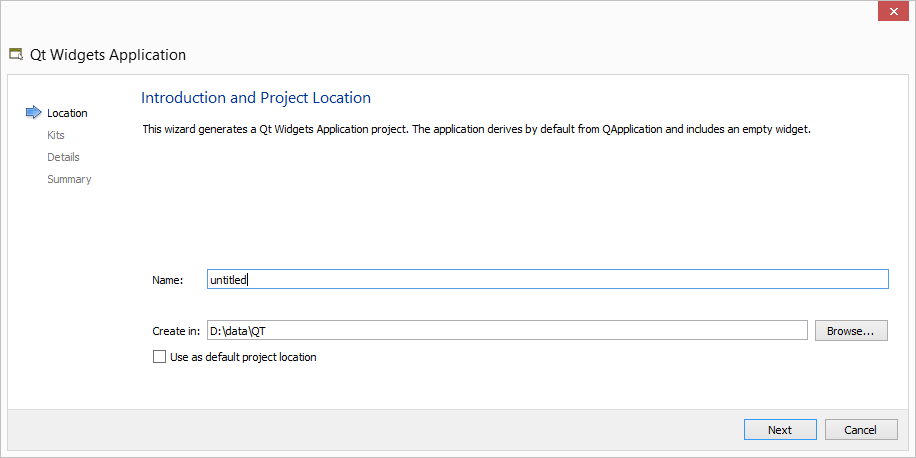
\includegraphics[width=0.8\textwidth]{../manuscript/images/Capture14-2.PNG}
		
		\item Pilih compiler yang di gunakan, jika mengginginkan aplikasi Cross Platform, maka sebaiknya menggunakan MinGW sebagai compilernya, tapi jika ingin aplikasi full support terhadap windows maka gunakan MSC.
		
		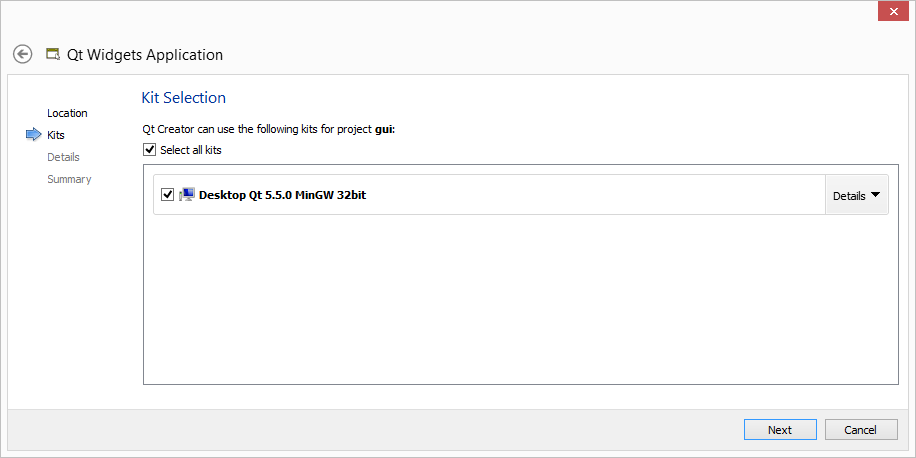
\includegraphics[width=0.8\textwidth]{../manuscript/images/Capture14-3.PNG}
		
		\item  Pada Class Information berikan nama class yang di gunakan, disini penulis menggunakan guibaru.
		
		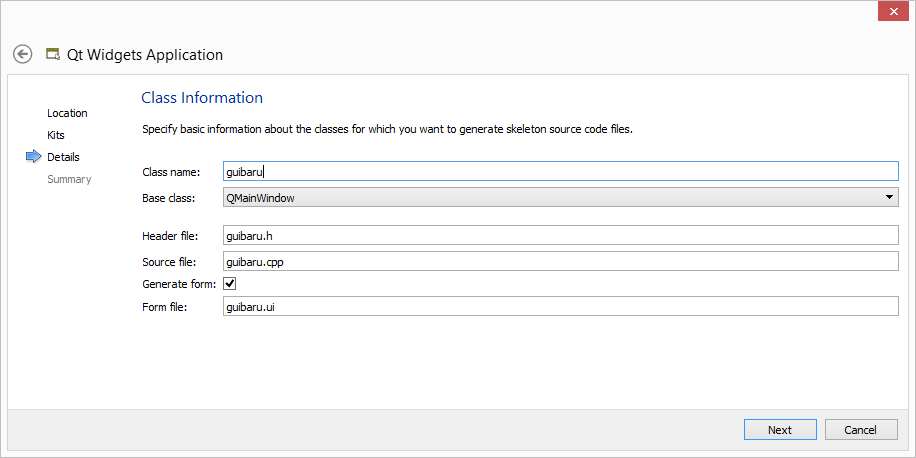
\includegraphics[width=0.8\textwidth]{../manuscript/images/Capture14-4.PNG}
		
		\item Kemudain langkah terakgir adalah project management, silahkan gunakan subversion\footnote{Anda bisa menggunakan Git, subversion, mercurial, bazaar, ClearCase, Perfoce atau CVS} yang Anda gunakan.
		
		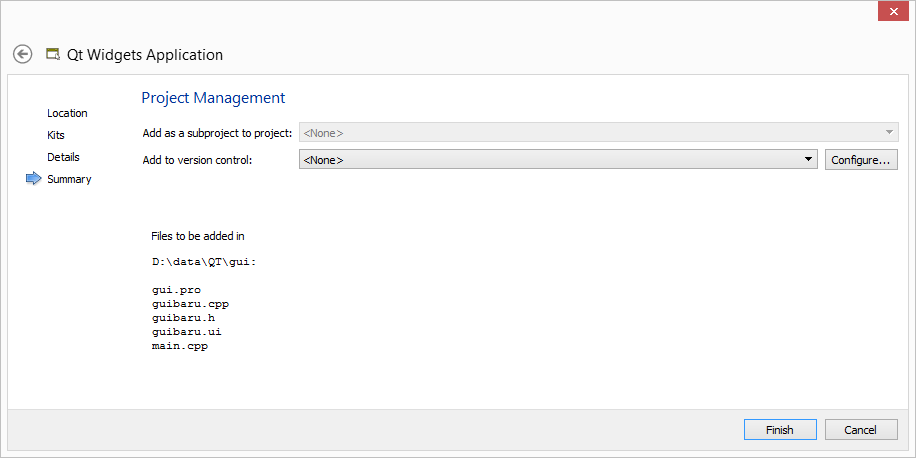
\includegraphics[width=0.8\textwidth]{../manuscript/images/Capture14-5.PNG}
		
		\item Finish, maka tampilan Qt Creator Anda akan seperti berikut ini
		
		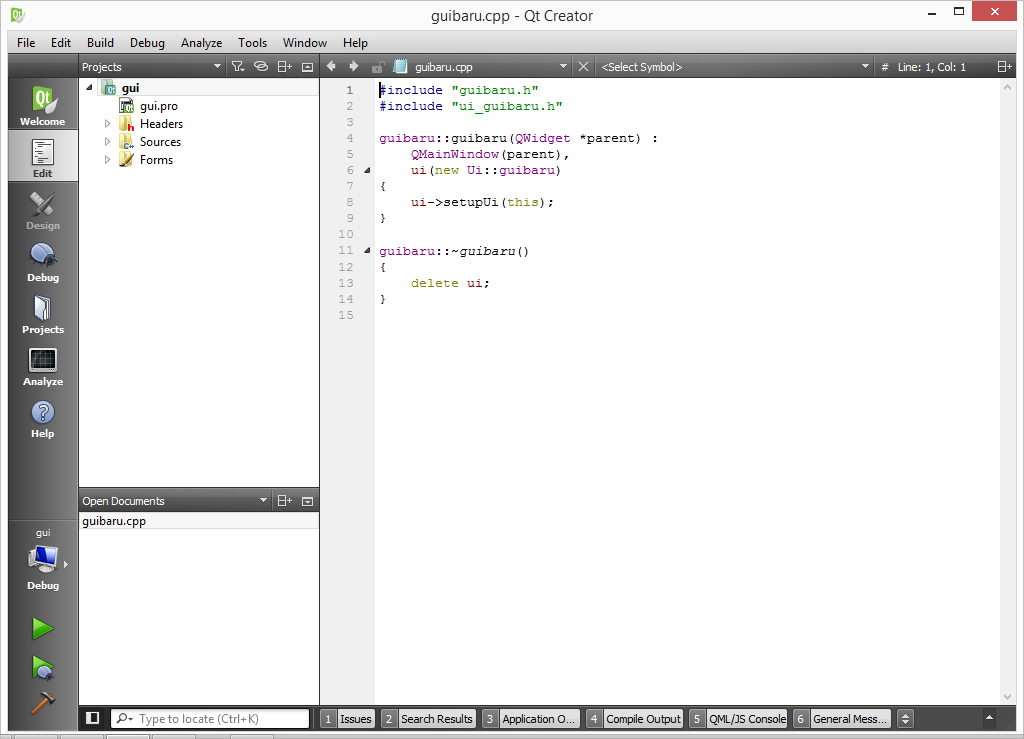
\includegraphics[width=0.8\textwidth]{../manuscript/images/Capture14-6.PNG}
		
		\item Perhatikan bahwa dalam proyek ini akan ada berkas yang terload secara otomatis oleh Qt creator yaitu
		
		\begin{itemize}
			\item \texttt{gui.pro} (berkas proyek Qt Creator yang bisa dipakai OS manapun)
			\item  \texttt{guibaru.cpp} (berkas kode inti tempat signal dan slot dituliskan)
			\item \texttt{guibaru.h} (berkas header)
			\item \texttt{guibaru.ui} (berkas GUI)
			\item \texttt{main.cpp} (berkas berisi fungsi yang selalu ada dalam semua program C/C++ yakni \texttt{main()})
			
		\end{itemize}
	
\end{enumerate}

\subsection{Membuat aplikasi}

\begin{enumerate}
	\item Buka \texttt{guibaru.ui}. guibaru.ui merupakan berkas XML Qt Creator, jika di klik maka GUI builder milik Qt Creator akan muncul.
	\item Drag dan drop Push button ke dalam layer kemudian doble klik pada label tersebut untuk membuat nama baru.
	
	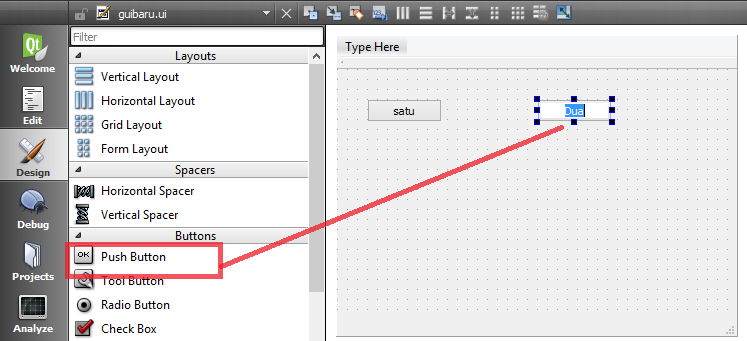
\includegraphics[width=0.8\textwidth]{../manuscript/images/Capture14-7.PNG}
	
	\item Berikan nama objek utuk label ini property panel di samping kanan. di bagian atas terdapat \texttt{QObjeck}. Tepat di bawahnya ada ObjeckName, pada label PushButton ganti dengan img.
	
	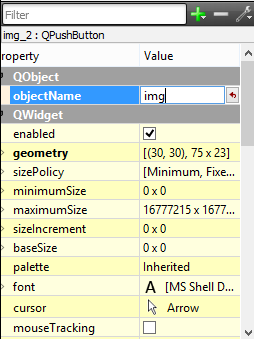
\includegraphics[width=0.8\linewidth, height=0.7\textheight]{../manuscript/images/Capture14-8.PNG}
	
	\item Di bagian a
	
\end{enumerate}